\documentclass[11pt]{article}
\usepackage[top=2cm,bottom=2cm,left=1.75cm,right= 1.75cm]{geometry}
%\geometry{landscape}                % Activate for for rotated page geometry
\usepackage[parfill]{parskip}    % Activate to begin paragraphs with an empty line rather than an indent
\usepackage{graphicx}
\usepackage{amssymb}
\usepackage{epstopdf}
\usepackage{amsmath}
\usepackage{multirow}
\usepackage{hyperref}
%\usepackage{changepage}
\usepackage{lscape}
%\usepackage{ulem}
\usepackage{multicol}
\usepackage{setspace}
\usepackage{dashrule}
\usepackage[usenames,dvipsnames]{color}
\usepackage{enumerate}
\usepackage{enumitem}
\newcommand{\urlwofont}[1]{\urlstyle{same}\url{#1}}
\newcommand{\degree}{\ensuremath{^\circ}}
\newcommand{\hl}[1]{\textbf{\underline{#1}}}
\newcommand\given[1][]{\:#1\vert\:}

% footnote citation
\usepackage[style=authortitle-ibid, maxnames=3,natbib=true,sortcites=true,block=space]{biblatex}
\bibliography{final}

% color hyperlinks
%\usepackage[colorlinks=false,pdfborder={0 0 0},urlcolor= MidnightBlue,colorlinks=true,linkcolor= MidnightBlue, citecolor= MidnightBlue,backref=true]{hyperref}

\DeclareGraphicsRule{.tif}{png}{.png}{`convert #1 `dirname #1`/`basename #1 .tif`.png}

\newenvironment{choices}{
\begin{enumerate}[(a)]
}{\end{enumerate}}

%\newcommand{\soln}[2]{\textcolor{MidnightBlue}{\textit{#2}}}{} 		% solutions
\newcommand{\soln}[2]{\vspace{#1}}{}						% exam, handout, etc.

%\newcommand{\solnMult}[1]{\textbf{\textcolor{MidnightBlue}{\textit{#1}}}}	% uncomment for solutions
\newcommand{\solnMult}[1]{ #1 }	% uncomment for handouts

%\newcommand{\tf}[1]{ \textbf{\textcolor{MidnightBlue}{\textit{#1}}} }	% uncomment for solutions
\newcommand{\tf}[1]{}	% uncomment for handouts

%\newcommand{\pts}[1]{ \textbf{{\small \textcolor{BurntOrange}{(#1)}}} }	% uncomment for solutions
\newcommand{\pts}[1]{ \textbf{{\small \textcolor{black}{(#1)}}} }	% uncomment for handouts

\newcommand{\note}[1]{ \textbf{\textcolor{red}{[#1]}} }	% uncomment for handouts

\newcommand{\qt}[1]{\textcolor{RoyalBlue}{\textbf{\textit{#1.}}}}

\renewcommand{\emph}[1]{\underline{\textbf{#1}}}

\newcommand{\reference}[1]{ \textbf{\textcolor{red}{[#1]}} }

%\newcommand{\fb}[3]{
%  \textcolor{NavyBlue}{\textbf{Question Feedback:} #1} \\$\:$\\
%  \textcolor{NavyBlue}{\textbf{This question refers to the following learning objective(s):}\\
%  \textbf{\textit{#2:}} #3}
%}


\begin{document}

\begin{titlepage}

\enlargethispage{\baselineskip}


STA 112 \hfill Dr. Evans \\
Spring 2022	\hfill Exam 2\\

\vspace{-2cm}

\begin{center}
{\Huge Exam 2}	
\end{center}

$\:$ \\

\textbf{Last Name:} \rule{5cm}{0.5pt}	\hfill	 \textbf{First Name:}  \rule{5cm}{0.5pt}	 \\
$\:$ \\
%\textbf{Section:} A (11 AM) $\quad$ B (9:30 AM) \hfill	
%\textbf{Team Name:}  \rule{7cm}{0.5pt} \\
$\:$ \\

\textit{I hereby state that I have not communicated with or gained information in any way from other students or any outside resource during this exam. I agree to abide by the rules stated below, and to abide by the Wake Forest Honor Code. All work is my own. I understand that any violation of this agreement will be reported to the Honor Council and will result, at minimum, in a 0 on this exam.}
\[ Signature: \rule{7cm}{0.5pt}\]

\hdashrule[0.5ex]{\textwidth}{0.5pt}{3mm}

\textbf{All work on this exam must be your own.}

{\small
\begin{enumerate}
\item You have 50 minutes to complete the exam.
\item Show all your work on the open ended questions in order to get partial credit. No credit will be given for open ended questions where no work is shown, even if the answer is correct.
\item You are allowed a calculator, however you may not share a calculator with another student during the exam. The calculator must be only a calculator, and may not be connected to the internet. 
\item You are allowed to ask clarification questions to me, but you may not ask anyone else. 
\item You are \hl{not} allowed a cell phone, even if you intend to use it as a calculator or for checking the time. You are \hl{not} allowed a music device or headphones, notes, books, or other resources. 
\item You may \hl{not} communicate with anyone other than myself during the exam.
\item Write clearly and be clear. Make it easy to find your answers. 
\end{enumerate}
}
\begin{center}
{\Large Good luck!}
\end{center}
\hdashrule[0.5ex]{\textwidth}{0.5pt}{3mm}

%\begin{center}
%\includegraphics[width=0.5\textwidth]{../figures/bubbles_new}
%\end{center}



\end{titlepage}

\pagebreak

%%%%%%%%%%%%%%%%%%%%%%%%%%%%%%%%%%%%%%%
$\:$ \\
\thispagestyle{empty}
\pagebreak

%%%%%%%%%%%%%%%%%%%%%%%%%%%%%%%%%%%%%%%
\setcounter{page}{1}
%%%%%%%%%%%%%%%%%%%%%%%%%%%%%%%%%%%%%%%

%\rule{\textwidth}{1pt}
%\begin{center}
%\textit{Answer questions \ref{DriveStart} to \ref{DriveEnd} based on the information %below.} \\
%\end{center}
\rule{\textwidth}{0.5pt}

\textbf{The Data} We have a client who is interested in examining which factors influence the fuel efficiency of different cars. The client is curious about the relationship between a car's \textit{engine displacement} (a measure of how big the engine is, measured in liters) and its fuel efficiency (measured in miles per gallon). The client also suspects fuel efficiency may be related to whether the car is front-wheel drive, rear-wheel drive, or four-wheel drive.

We have information on 234 different cars, and the following three variables:

\begin{itemize}
\item \texttt{mpg}: the car's fuel efficiency, in miles per gallon
\item \texttt{displacement}: the car's engine displacement (size), in liters
\item \texttt{drive}: either front-wheel, rear-wheel, or four-wheel
\end{itemize}

Below are side-by-side boxplots showing the distribution of fuel efficiency for each drive type.

\begin{center}
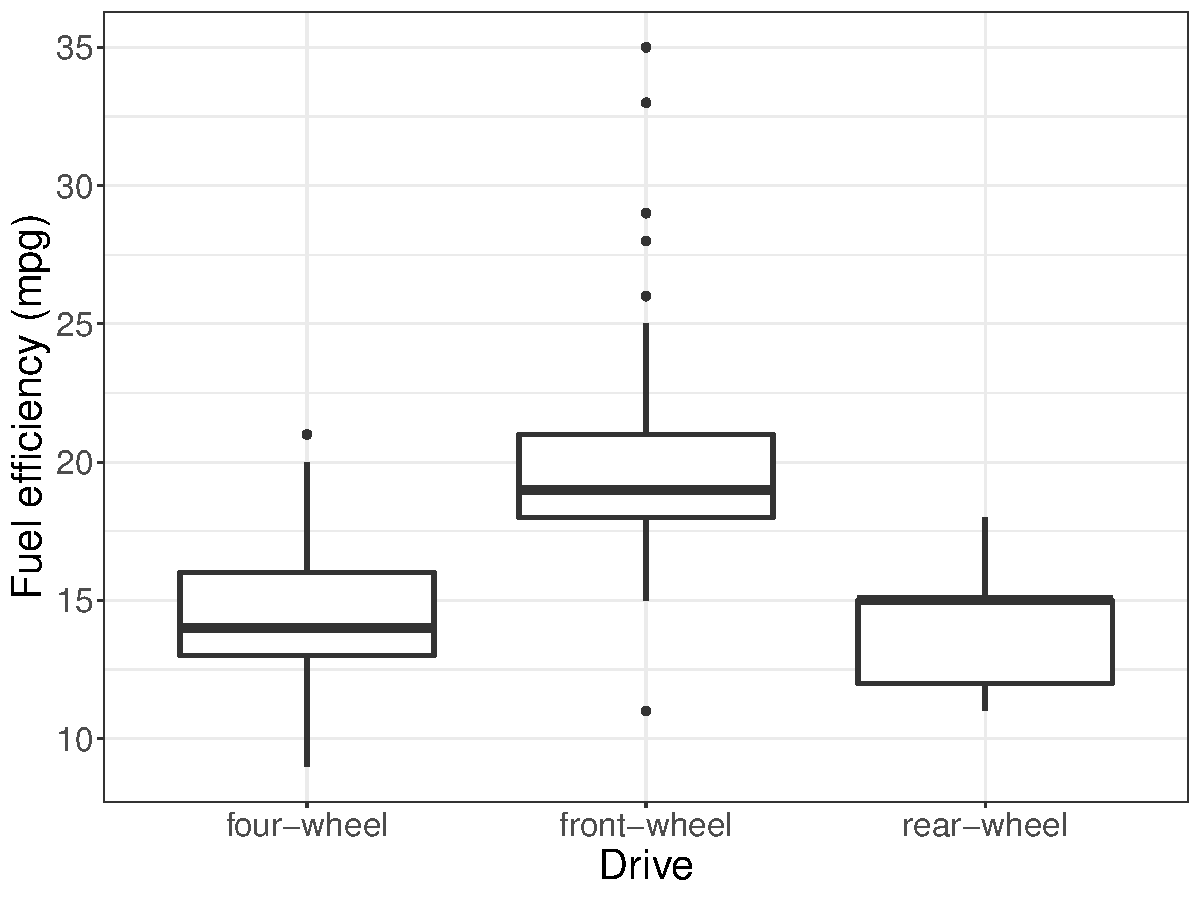
\includegraphics[scale=0.7]{exam2_fig1.pdf}
\end{center}

\rule{\textwidth}{1pt}

\pagebreak

\rule{\textwidth}{1pt}

We will begin by looking at the relationship between drive type and fuel efficiency.

\rule{\textwidth}{1pt}

\begin{enumerate}

\item Write down a population model with drive type as the predictor, and fuel efficiency as the response. Use appropriate notation. (Ignore engine displacement for now).

\vspace{4cm}

\item The client fits your model, resulting in the following model output. Using the fitted model, report the estimated average fuel efficiency for cars of each drive type (four-wheel, front wheel, and rear-wheel).

\vspace{1cm}

\begin{center}
\begin{tabular}{rrrrr}
  \hline
             & Estimate & Std. Error \\
  \hline
(Intercept)    & $14.33$ & $0.314$    \\
 driveFrontWheel    & $5.64$ & $0.442$ \\
 driveRearWheel & $-0.25$ & $0.71$ \\
  \hline
\end{tabular}
\end{center}

\vspace{4cm}

\item The client wants to test whether there is a relationship between drive type and fuel efficiency. Using your model from Question 1, write down null and alternative hypotheses, in terms of one or more model parameters, for this research question. 

\pagebreak

\item To test the hypotheses from Question 3, your client starts to create an ANOVA table. Unfortunately, after filling in the sums of squares, the client gets stuck. Help them out by filling in the rest of the ANOVA table. (You can write the table separately if you need more space).

\begin{center}
\begin{tabular}{|c|c|c|c|c|}
\hline
\textbf{Source} & \textbf{degrees of freedom (df)} & \textbf{Sum of Squares (SS)} & \textbf{Mean Squares (MS)} & \textbf{F} \\
\hline
Model & & 1878.8 & & $\hspace{1.5cm}$ \\
Residual & & 2341.5 & &  \\
\hline
Total & & & & \\
\hline
\end{tabular}
\end{center}

\pagebreak

\item Using your ANOVA table, what is the value of the test statistic you will use to test your hypotheses from Question 3? What distribution will you compare your test statistic with to calculate a p-value (give the name and degrees of freedom for the distribution).

\vspace{3cm}

\item The test statistic you calculated corresponds to the data shown in the boxplots on page 1. What could those boxplots look like if the test statistic in Question 5 was \textit{smaller}? Draw a sketch, and explain your reasoning.

\pagebreak

\rule{\textwidth}{1pt}

The client is now interested in adding engine displacement to the model. In particular, the client wants to know whether a change of 1 liter in engine displacement is associated with the same change in fuel efficiency for four-wheel drive cars, front-wheel drive cars, and rear-wheel drive cars (i.e., is the relationship between displacement and fuel efficiency the same for each drive type).

\rule{\textwidth}{1pt}

\item Write down a population model that allows the client to answer this research question. Use appropriate notation, and explain your reasoning for choosing the model.

\vspace{5cm}

\item The client fits your model, resulting in the following model output. Interpret the fitted coefficient $-2.07$ in context.

\begin{center}
\begin{tabular}{rrrrr}
  \hline
             & Estimate & Std. Error \\
  \hline
(Intercept)    & $22.59$ & $0.814$    \\
 driveFrontWheel    & $6.13$ & $1.163$ \\
 driveRearWheel & $-3.01$ & $3.104$ \\
 displacement & $-2.07$ & $0.196$ \\
 driveFrontWheel:displacement & $-1.35$ & $0.370$ \\
 driveRearWheel:displacement & $1.00$ & $0.605$ \\
  \hline
\end{tabular}
\end{center}

\pagebreak

\item The client wants to know whether a change of 1 liter in engine displacement is associated with the same change in fuel efficiency for each drive type. Using your model from Question 7, write down null and alternative hypotheses, in terms of one or more model parameters, for this research question.

\vspace{3cm}

\item Which test should the client use to test these hypotheses? (nested F test, t test, or either?) Explain your reasoning, and give the degrees of freedom for the test.

\vspace{3cm}


\item Now you want to check assumptions to make sure your hypothesis tests are valid. Explain to the client which diagnostic plot you will use to assess the shape and constant variance assumptions. Then, sketch an example diagnostic plot in which both the shape \textit{and} constant variance assumptions are violated. Make sure to label the axes.


\pagebreak

\rule{\textwidth}{1pt}

To compare nested regression models we use a nested F test, where the test statistic is given by

$$F = \dfrac{\frac{1}{\# \text{parameters tested}} (SSE_{reduced} - SSE_{full})}{\frac{1}{n-p} SSE_{full}}$$

where $n$ is the number of observations in the data, and $p$ is the number of parameters in the full model. $SSE_{reduced}$ and $SSE_{full}$ are the residual sum of squares for the reduced and full models; recall that

$$SSE = \sum \limits_{i=1}^n (y_i - \widehat{y}_i)^2 \hspace{1cm} SSModel = \sum \limits_{i=1}^n (\widehat{y}_i - \overline{y})^2 \hspace{1cm} SSTotal = \sum \limits_{i=1}^n (y_i - \overline{y})^2 $$

and $SSTotal = SSModel + SSE$.

\rule{\textwidth}{1pt}


\item The F test you calculated with the ANOVA table in Question 4 is a special case of the nested F test, when we are testing whether there is a relationship between a single categorical predictor and a quantitative response. Using the formula for the nested F statistic given here, explain why.

\pagebreak

%%%%%%%%%%%%%%%%%%%%%%%%%%%%%%%%%%%%%%%%


\huge{You are done!!! Whooo!!!}


%%%%%%%%%%%%%%%%%%%%%%%%%%%%%%%%%%%%%%%%


\end{enumerate}

%%%%%%%%%%%%%%%%%%%%%%%%%%%%

%\pagebreak

%\hdashrule[0.5ex]{\textwidth}{0.5pt}{3mm}
%\begin{center}
%\renewcommand{\arraystretch}{1.5}
%\begin{tabular}{| l | c | c | c | c | c | c  || c |}
%\hline
%				& 		& 		& 		& 		&	&  	&\\
%				& Q1-Q3		& Q4-6		& Q7		& Q8-Q10		 & Q11-Q12	 & Q13 & Total	\\
%\hline
%Points earned		& \textcolor{white}{xxxxx} &	\textcolor{white}{xxxxx}	& \textcolor{white}{xxxxx}	&	\textcolor{white}{xxxxx}&%\textcolor{white}{xxxxx}	&	\textcolor{white}{xxxxx} &	\textcolor{white}{xxxxx} \\
%\hline
%Available points	& 9 		& 12		& 9		& 9		&7 & 4 					& 50 \\
%\hline
%\end{tabular}

%\end{center}

\end{document}
